\chapter{Generalized Angularities}
\label{ch:angularities}

Generalized jet angularities are a family of jet observables defined as,

\begin{equation}\label{eq:LambdaKappaBeta}
	\lambda_\beta^\kappa=\sum_{\mathrm{const} \in \mathrm{jet}}\left(\frac{p_{\rm T, const }}{p_ {\rm T,  jet}}\right)^\kappa \left(\frac{\Delta R_\mathrm{const, jet}}{R}\right)^\beta
\end{equation}

where \Pt{jet/const}~is the jet/constituent's momentum, and \(\Delta R_\mathrm{const, jet}\) is the \etaphi distance of a constituent from the jet-axis given by, 

\begin{equation}
		\Delta R_\mathrm{const, jet} = \sqrt{(\eta_{\rm jet}-\eta_{\rm const})^2 + (\phi_{\rm jet}-\phi_{\rm const})^2}
\end{equation}

Parameters $\kappa$ and $\beta$ tune experimental sensitivity to hard and wide-angle radiation, respectively. $\lambda^1_\beta$'s are infra-red and collinear (IRC) safe angularites~\cite{Larkoski_2014}, which probe the average angular spread of energy around the jet-axis. They are radial moments of the  jet's transverse momentum profile, also known as differential jet-shape (\(\pi_T(\mathbf{r})\)), given by,

\begin{equation}\label{eq:RhoRIntro}
	\pi_T(\mathbf{r}) = \lim_{\delta r \rightarrow0}\Big\langle\frac{1}{\delta r}\frac{\sum_{|\mathbf{r_{\rm const}} - \mathbf{r}|<\delta r/2}p_{\rm T, const}}{p_{\rm T,  jet}}\Big\rangle _{\rm jets} ,
\end{equation}
where  $\mathbf{r}_{\rm const} =  (\eta_{\rm const}-\eta_{\rm jet})\hat{\eta}+ (\phi_{\rm const}-\phi_{\rm jet})\hat{\phi}$, and it follows that, 
\begin{equation}
	\lambda_\beta^1 = \int_{\rm jet} r^\beta\pi_T(\mathbf{r}) d\mathbf{r} .
\end{equation} 

However, as an experimental observable, it is useful to restrict the summation in Eq. \ref{eq:LambdaKappaBeta} to only charged constituents / tracks and mitigate contamination from towers like pileup.  This comes at the cost of IRC safety of \(\lambda_\beta^1\) as theoretical predictions will involve non-perturbative fragmentation functions. 




\section{Angularities of \(p + p\) jets}
The analysis uses data from \pp collisions at \sPP{200}{GeV}~collected in 2012 using the STAR detector system. Charged-particle tracks and neutral energy depositions (towers) are measured using STAR's Time Projection Chamber (TPC) \cite{Anderson_2003} and Barrel Electromagnetic Calorimeter (BEMC) \cite{BEDDO2003725} detectors respectively. 

To enhance jet signal, only High-Tower (HT) triggered events, with at least one tower with $\EtTower \geq 4$ GeV are considered. Events containing a track with \ptGeq{track}{30} are rejected to avoid contamination from cosmic rays. Tracks(Towers) with \ptGeq{track}{0.2} (\(E_\mathrm{T, tower} \geq 0.2\) GeV) are considered for jet clustering. Clustered jets completely falling within acceptance ($|\eta_{\rm jet}| \leq 0.6$), with \ptGeq{jet}{10} and a plurality of charged tracks (\(N_\mathrm{ch., jet} \geq 2\)) are used for further study.  
%Jets with area, $A_{\rm jet} < 0.3$ are rejected to further reduce the fake jet contribution. 

 The tracks and towers are clustered into jets using the anti-\(k_{\rm T}\) algorithm with a jet resolution parameter $R = 0.4$, implemented using the FastJet library~\cite{Cacciari_2012}.  After obtaining the jets, the softer constituents are groomed using Recursive SoftDrop with \(\beta = 0\) and \(z_\mathrm{cut} = 0.2\). The groomed-jet's constituents lose non-kinematic information like charge, which is regained by matching them to the original jet's constituents. 
 
 \subsection{Detector effects and Unfolding}
 The embedding simulation starts from PYTHIA6 (STAR Tune)  at the particle level. The particles are then reconstructed as detector hits using the STAR detector system implemented in GEANT3 and embedded into zero-bias events from 200 GeV \pp collisions (2012). The jets from particle and detector levels are matched using a \(p_\mathrm{T, jet}\) ordered nearness criteria.  The matched jets can be used to show detector responses like shown in Fig. \ref{fig:PtResonse} and  \(p_\mathrm{T, jet}\)-resolution shown in fig.~\ref{fig:PtResolution}.  
 
 \begin{figure}[h]
 	\centering
 	\label{fig:PtResonse}
 	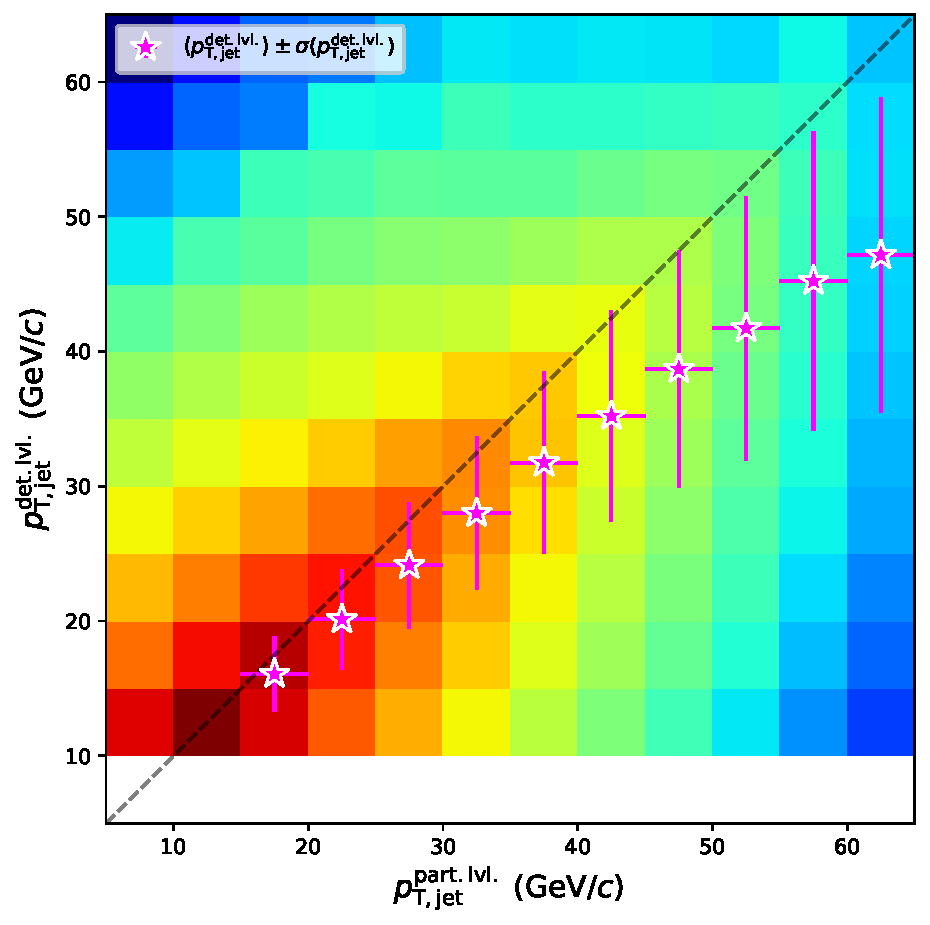
\includegraphics[width=0.5\linewidth]{figures/jet_pt_response.pdf}
 	\caption{Two-dimensional histogram showing detector response for \(p_\mathrm{T, jet}\), showing probability of a \ptGenJet particle level jet being reconstructed as \ptRecoJet. Purple stars shows expected \ptRecoJet given a particular bin of the \ptGenJet.}
 \end{figure}

 \begin{figure}[h]
 	\centering
 	\label{fig:PtResolution}
 	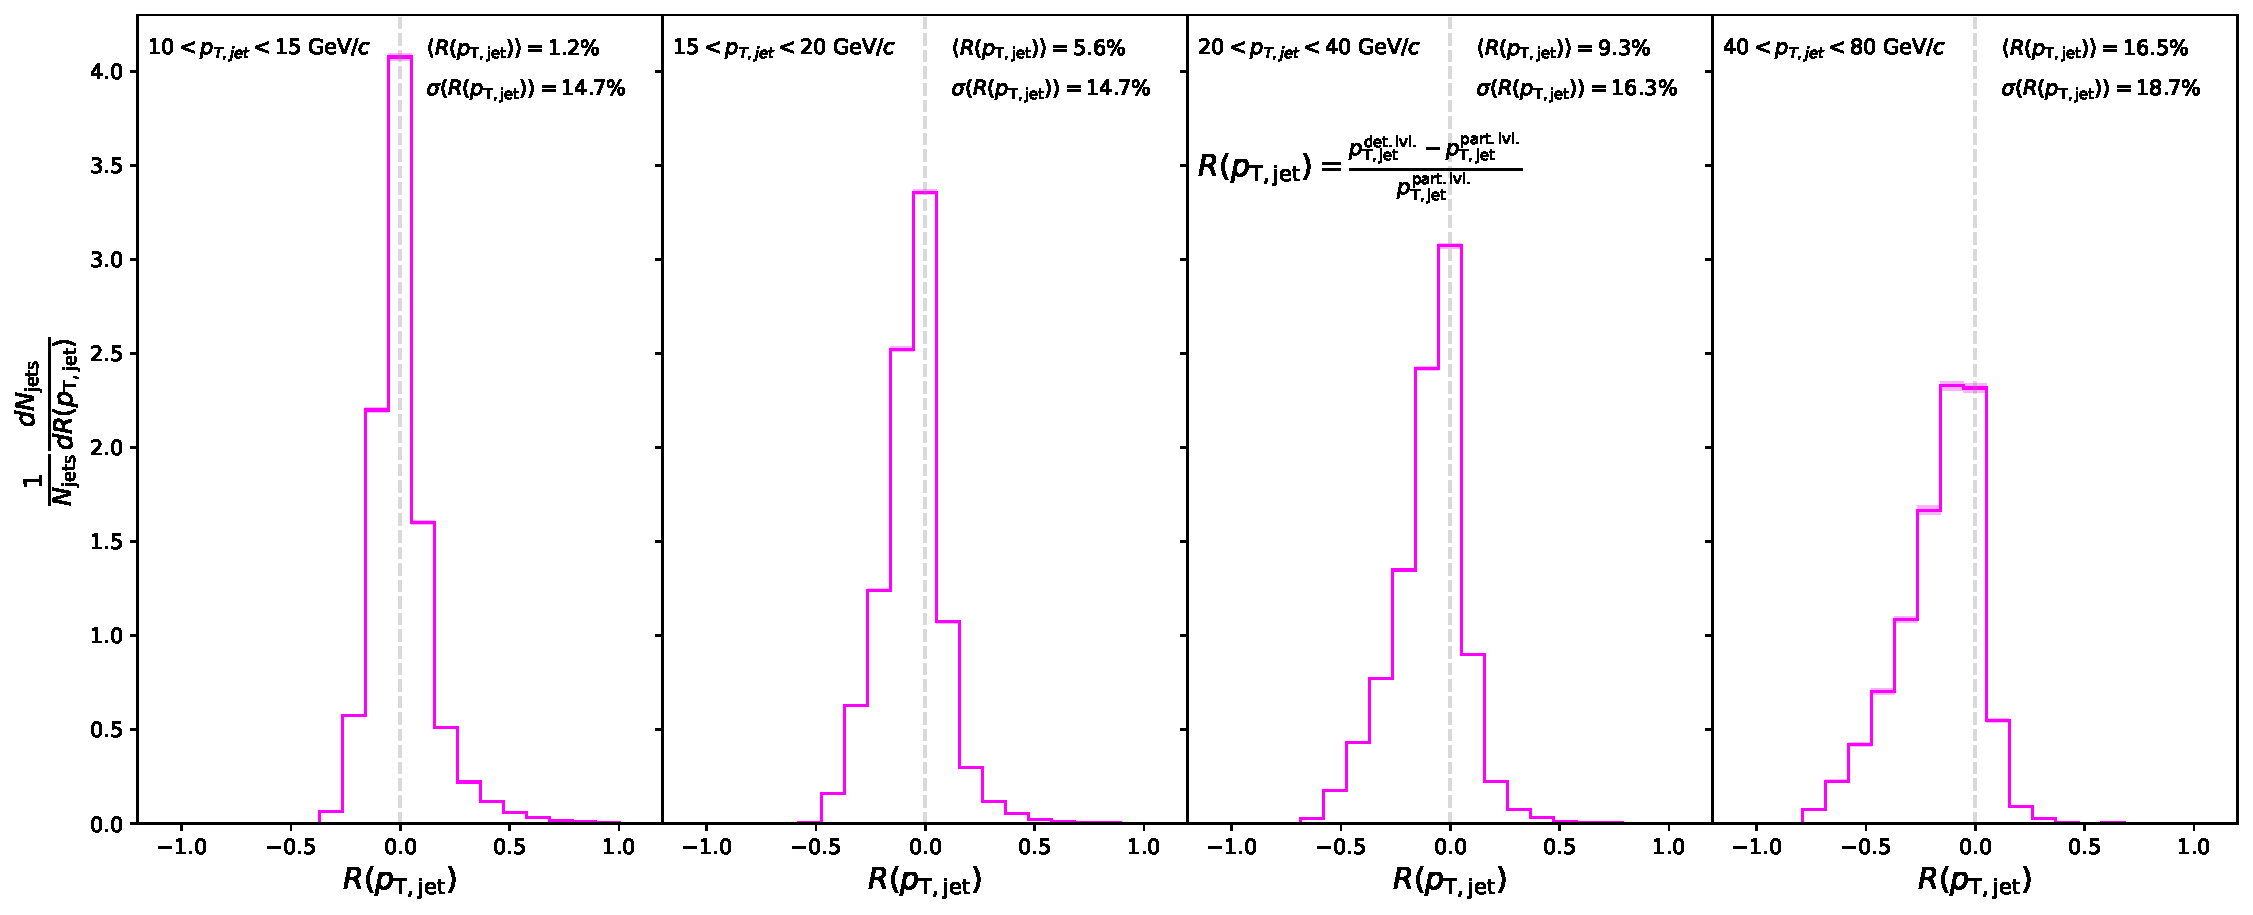
\includegraphics[width=\linewidth]{figures/jet_pt_res.pdf}
 	\caption{\(p_\mathrm{T, jet}\)-resolution in different \(p_\mathrm{T, jet}\) bins.}
 \end{figure}
 
 Unfolding is done using the Multifold method. Every jet is represented as a vector of 23 features. The four classifiers of Multifold are parametrized as DNNs with 3 hidden layers with 256 nodes each. The model weights are trained using the AdamW optimizer with a learning rate of \(10^{-3}\) and weight decay of \(10^{-2}\). Convergence is achieved in two unfolding iterations. Statistical uncertainties are calculated using bootstrap ensemble with 50 model replicas each sub-sampling  500k each of the data-like and sim-like jets, so each model replica sees 1M jets every epoch. All the  required unfolded distributions and profiles are calculated by using the per-jet unfolding weights. 
 
 Closure test of the unfolding shown in  Fig. \ref{fig:ClosureAngularity} and \ref{fig:ClosureAngVsRg} is done by doing the same unfolding procedure replacing measured data with pseudo-data for which the particle level is known (pseudo-truth). The pseudo-unfolded distributions are then compared to the pseudo-truth via ratios
 \begin{figure}[h]
 	\centering
 	\label{fig:ClosureAngularity}
 	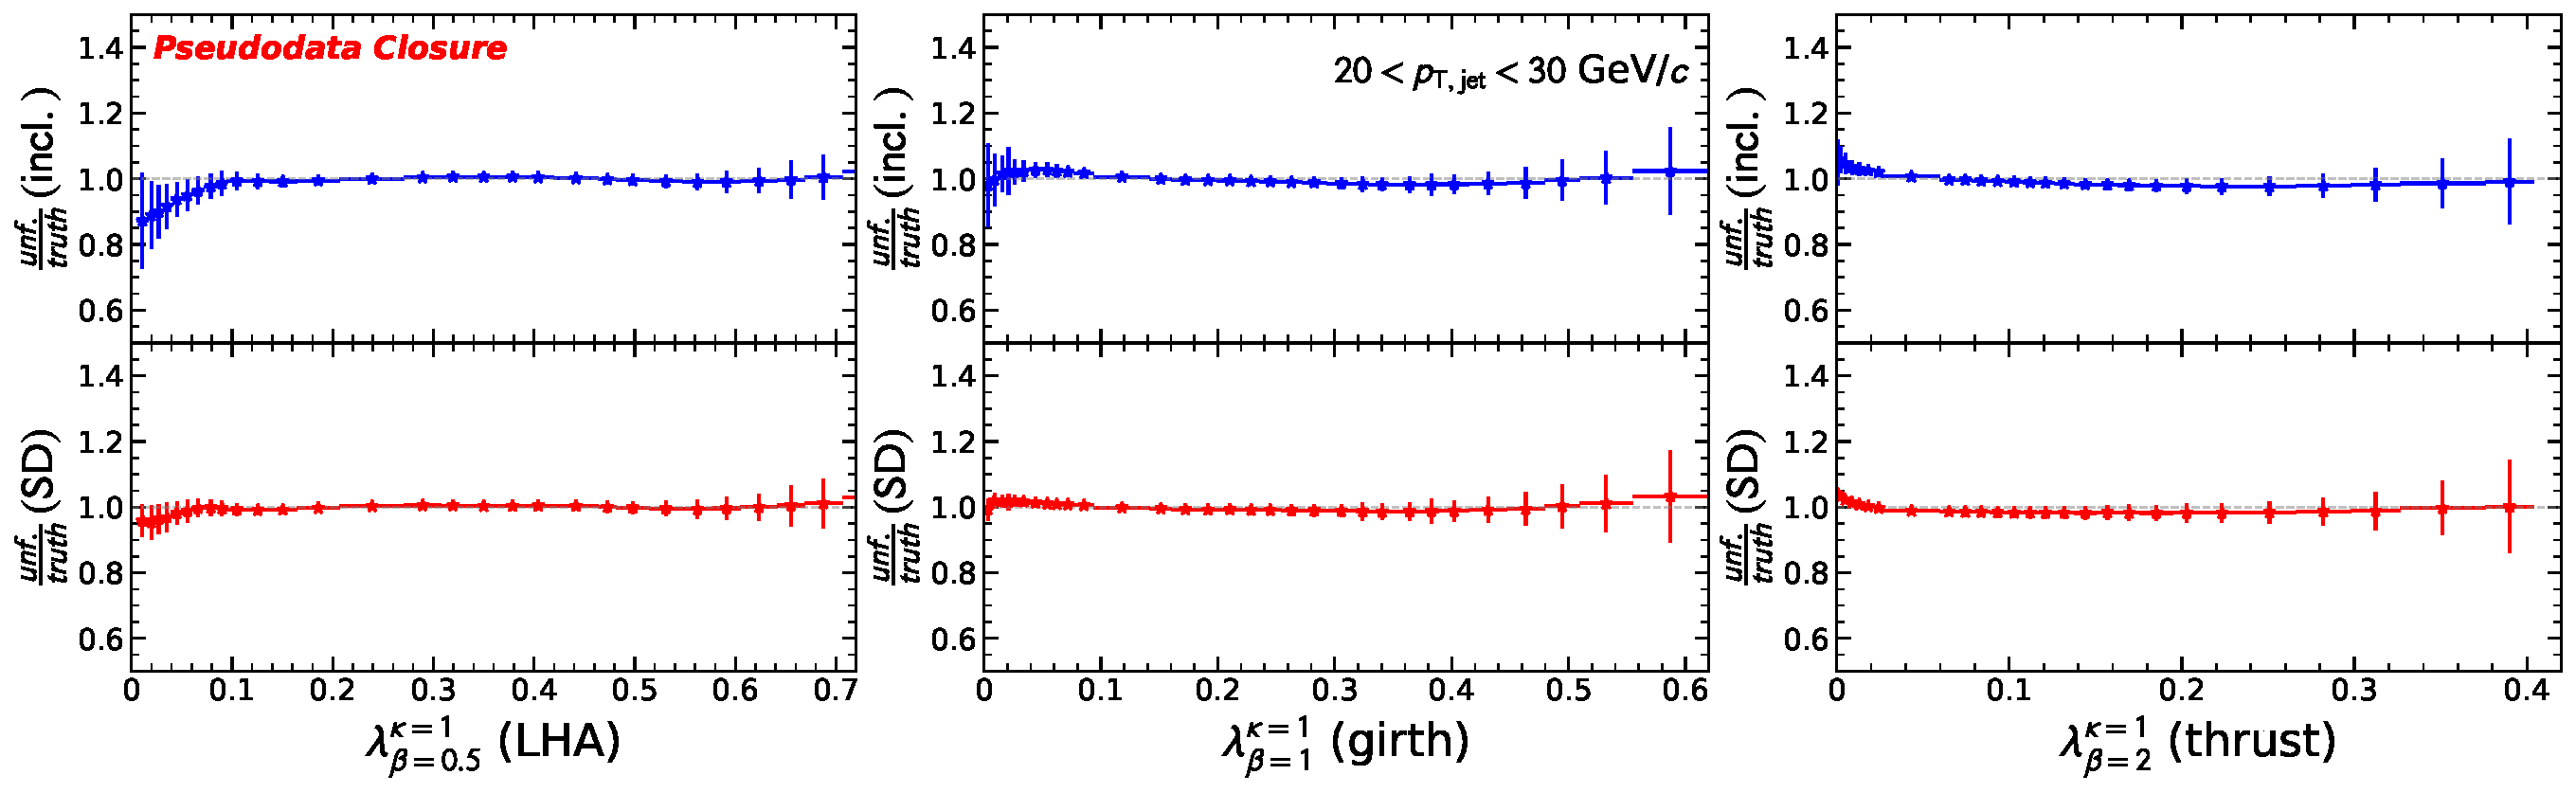
\includegraphics[width=\linewidth]{figures/fig_dist_grid_closure_like.pdf}
 	\caption{Closures for \(\lambda^{\kappa=1}_{\beta\in\{0.5, 1, 2\}}\) distributions.}
 \end{figure}
 
 \begin{figure}[h]
 	\centering
 	\label{fig:ClosureAngVsRg}
 	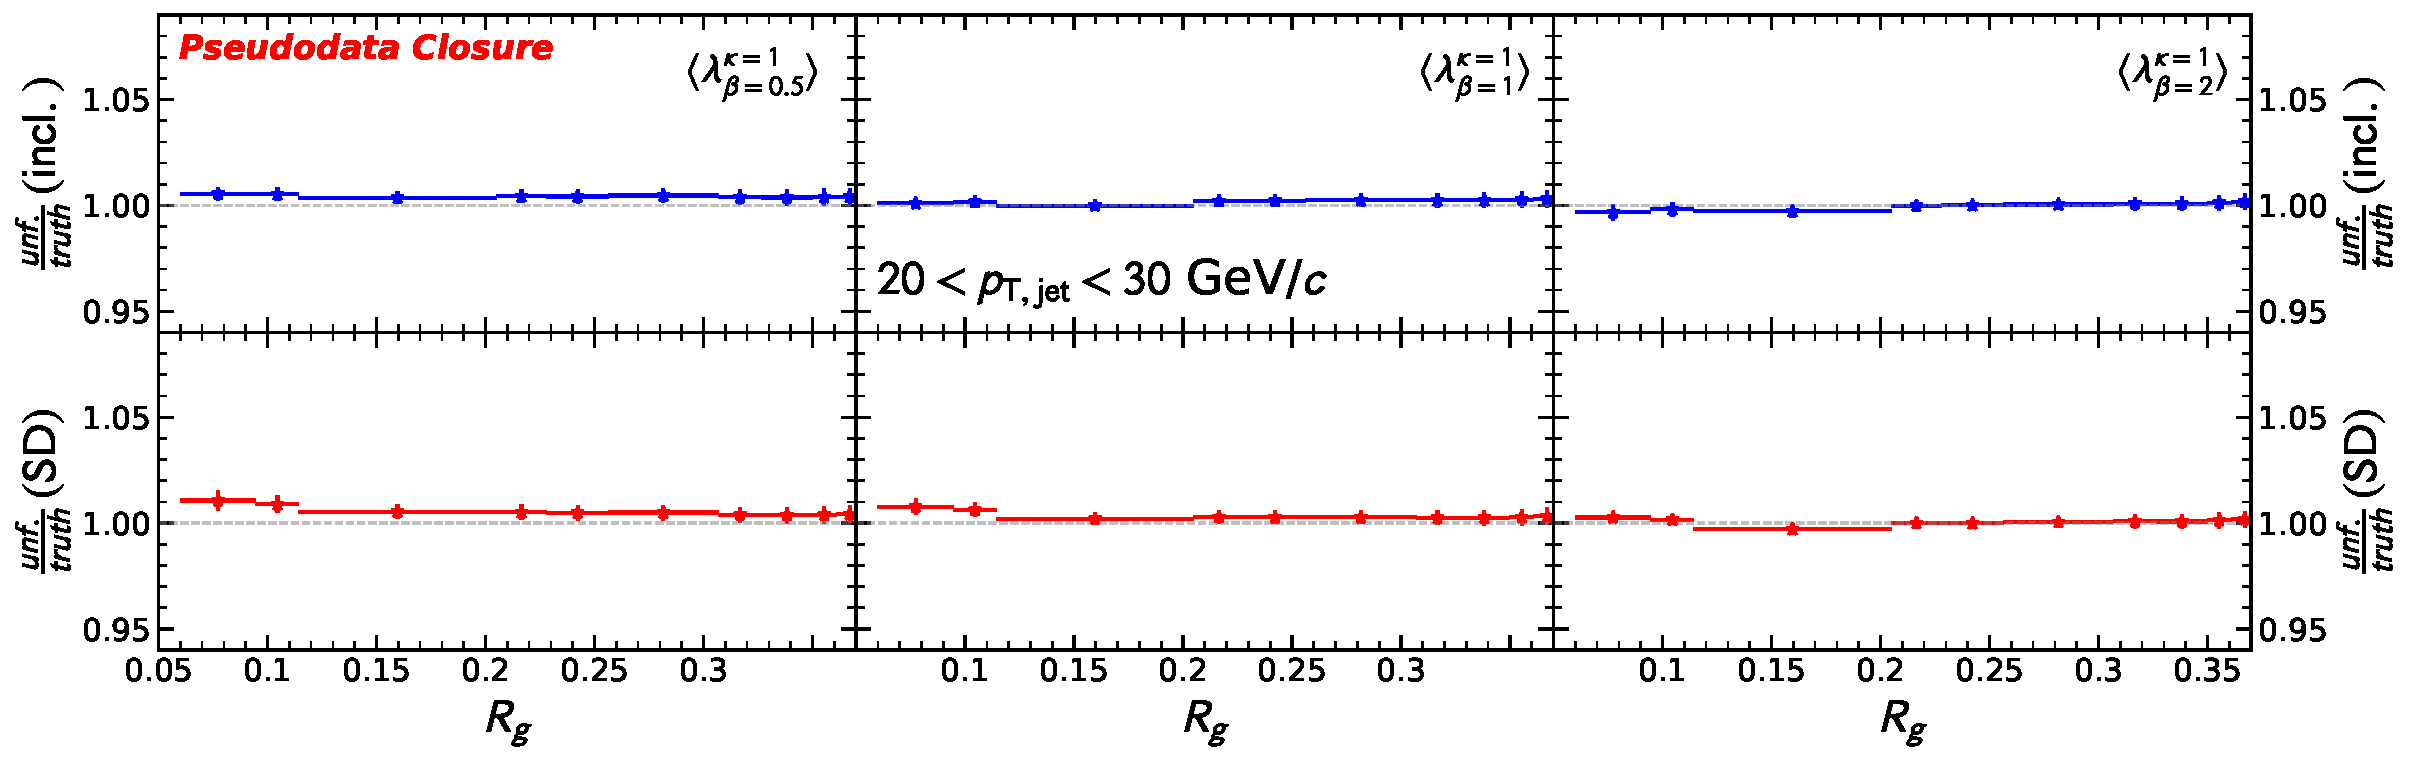
\includegraphics[width=\linewidth]{figures/fig_dr_grid_closure_like.pdf}
 	\caption{Closures for \(\lambda^{\kappa=1}_{\beta\in\{0.5, 1, 2\}}\) vs \(R_\mathrm{g}\) profile shown for jets with \ptRange{jet}{20}{40}.}
 \end{figure}
 
 \subsection{Systematic Uncertainties}
 \subsubsection{Jet Reconstruction Related Uncertainties}
 Analysis was rerun with each of the following changes (compared to the nominal) done to the detector level of the embedding simulation.  
 %
 The differences in the final plots for the source was calculated. 
 %
The Barlow test was performed on each source of systematic error to remove the statistical fluctuation from the variation.

 \begin{itemize}
 	\item Tracking Efficiency -  The uncertainty in tracking efficiency is estimated at $\pm 4 \%$ for \(p+p\) events.
 	\item Variation of Hadronic Correction - For the towers, we remove the full contribution of the track momentum for our central values. As a variation on that, we remove half of the total track momentum contribution.
 	\item Tower Gain Uncertainty - Tower energies increased by 3.8\%
 	\item \(p_\mathrm{T, jet}\) resolution - Use the \(p_\mathrm{T, jet}\) resolution values from fig.~\ref{fig:PtResolution} to shift the \(p_\mathrm{T, jet}\) windows in which results are presented. 
 \end{itemize}
 
 \subsubsection{Unfolding related uncertainties}
 \begin{itemize}
 	\item Variation of the regularization parameter(number of iterations) -  For our central values, we have used 2 iterations as we found the result to converge reliably by that point. We vary the iterations between 3 and 5.
 	\item Prior variation - Varied the prior of the embedding sample from PYTHIA6 to HERWIG7
 	\item Non Closure - Any deviations from 1 for ratios shown in fig.~\ref{fig:ClosureAngularity} and fig.~\ref{fig:ClosureAngVsRg}
 \end{itemize}
 
\subsection{Results and Discussions}
The \(\lambda_{\beta\in\{0.5,1,2\}}^{\kappa=1}\) distributions are showin in Figs.
%
Grooming shifts  the distributions to smaller angularity values. 
%
On average higher-\(\beta\) angularities are more affected by grooming, as contributions from early, soft, wide-angle radiation are more significant. 
 

The \(\langle\lambda^{\kappa=1}_\beta\rangle\) vs \(R_\mathrm{g}\) plots are shown in figs. 
%
$\langle\lambda^{\kappa=1}_\beta\rangle$ rises monotonically with $R_{\rm g}$, steepening with $\beta$. 
%
Shows angular ordering as high-$R_{\rm g}$ jets are unaffected by grooming, since widest split already passes $z_{\rm cut}$
%
The distributions and \(R_\mathrm{g}\) profiles are generally well explained within statistical/systematic uncertainties by PYTHIA-6, PYTHIA-8 and HERWIG-7.

\begin{figure}[h]
	\centering
		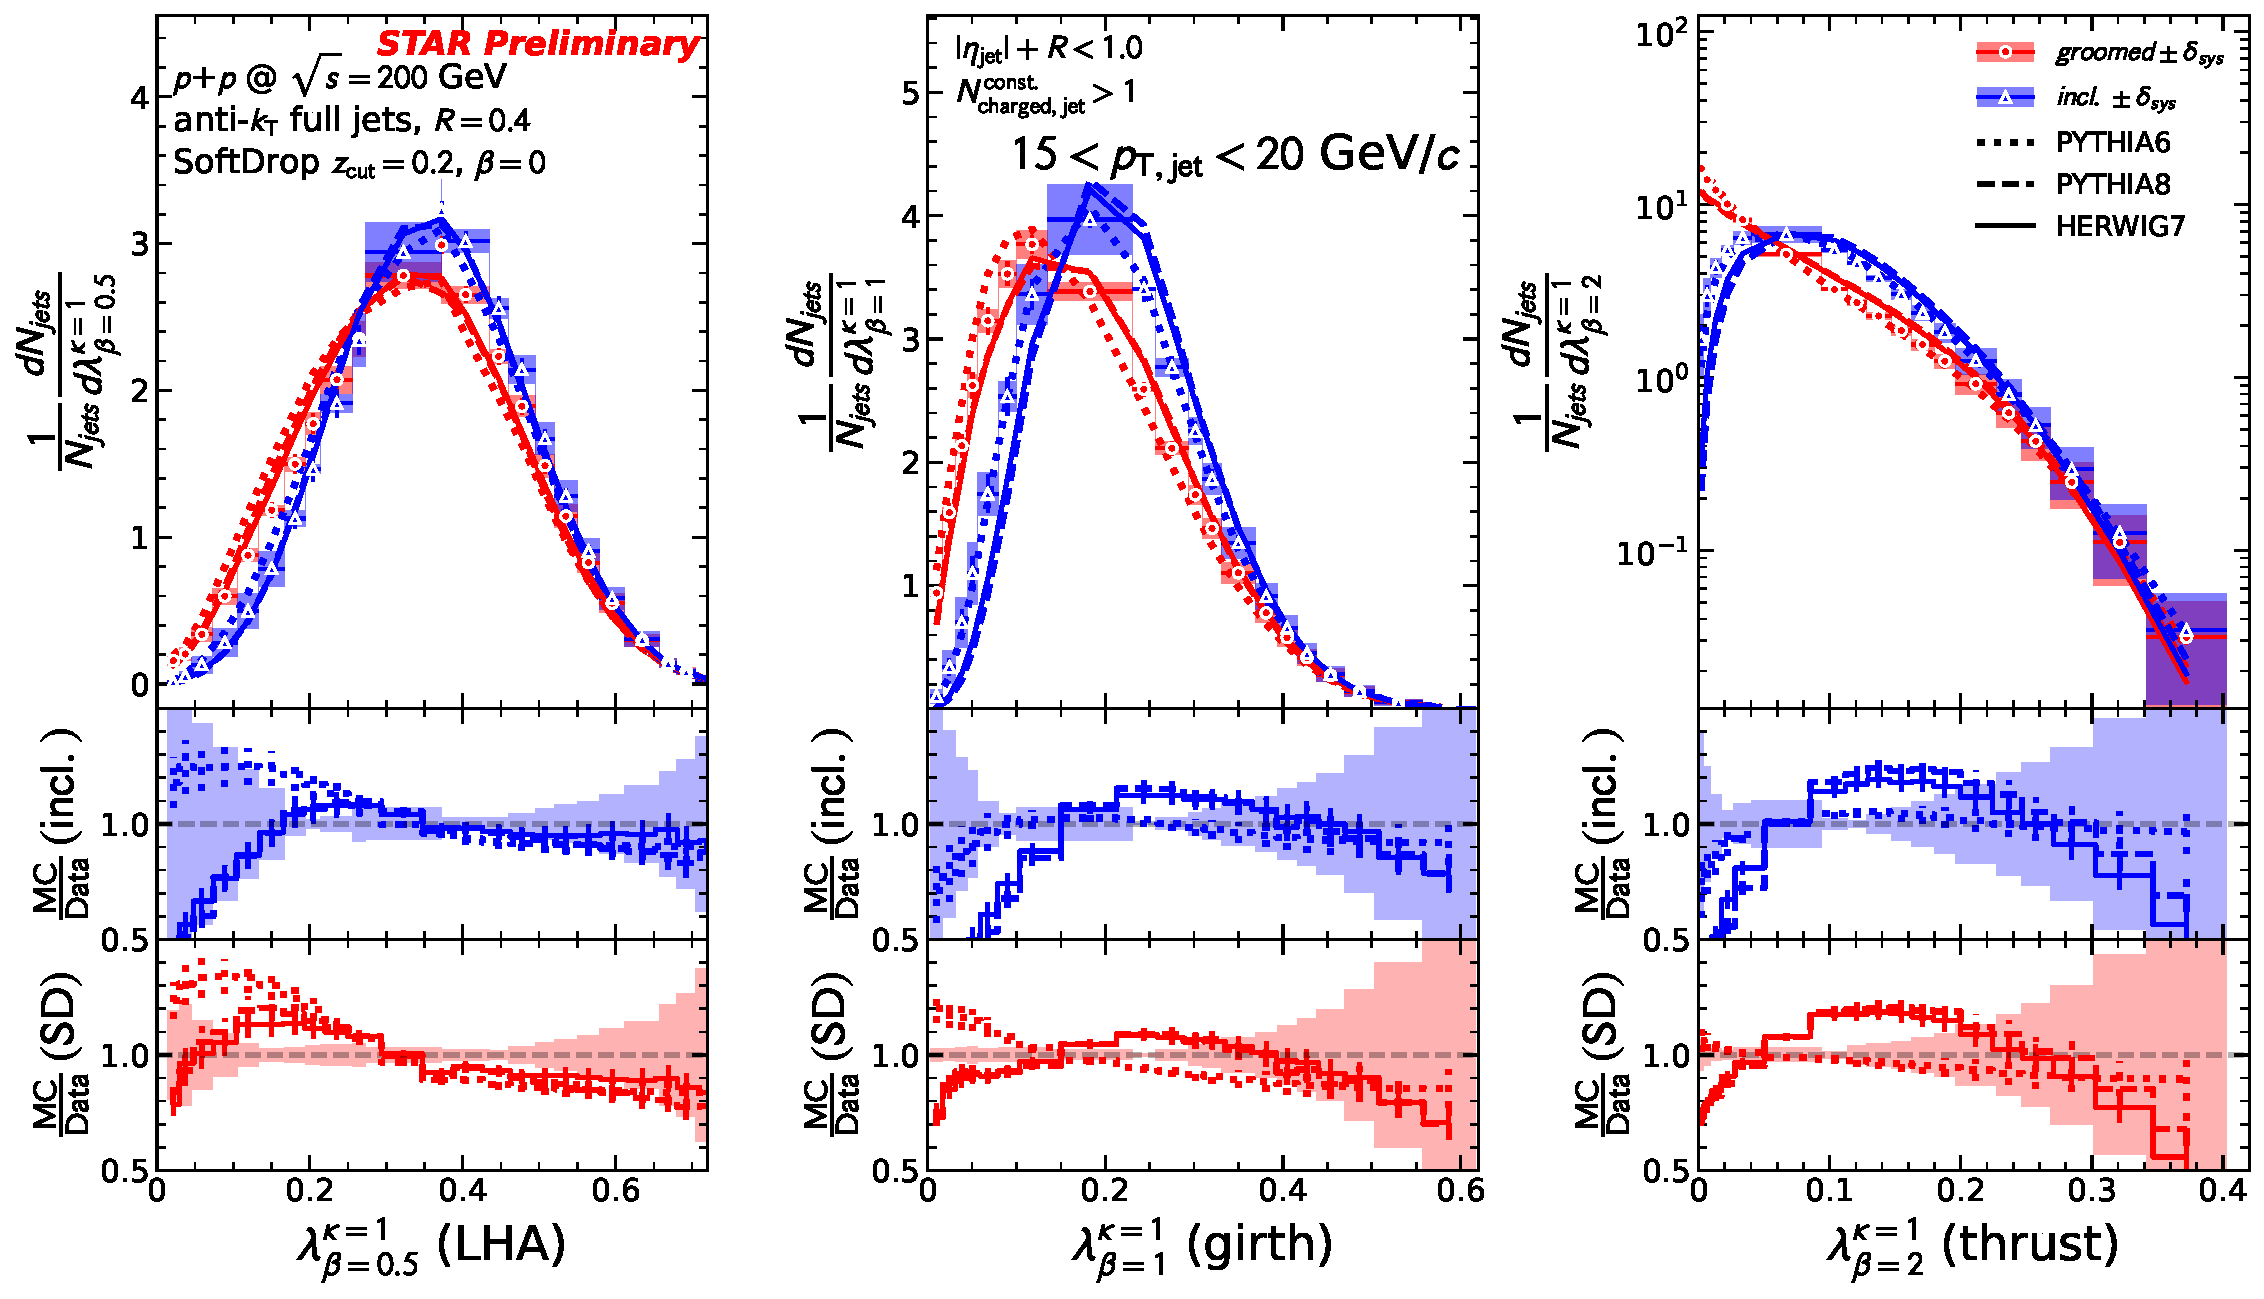
\includegraphics[width=\linewidth]{figures/fig_grid_jpt1.pdf}
		\caption{Distributions of \(\lambda_\beta^1\) for \(\beta = 0\) (left), \(\beta = 1\) (middle) and \(\beta = 2\) (right) for jets with \ptRange{jet}{15}{20}. }
\end{figure}
\begin{figure}[h]
	\centering
	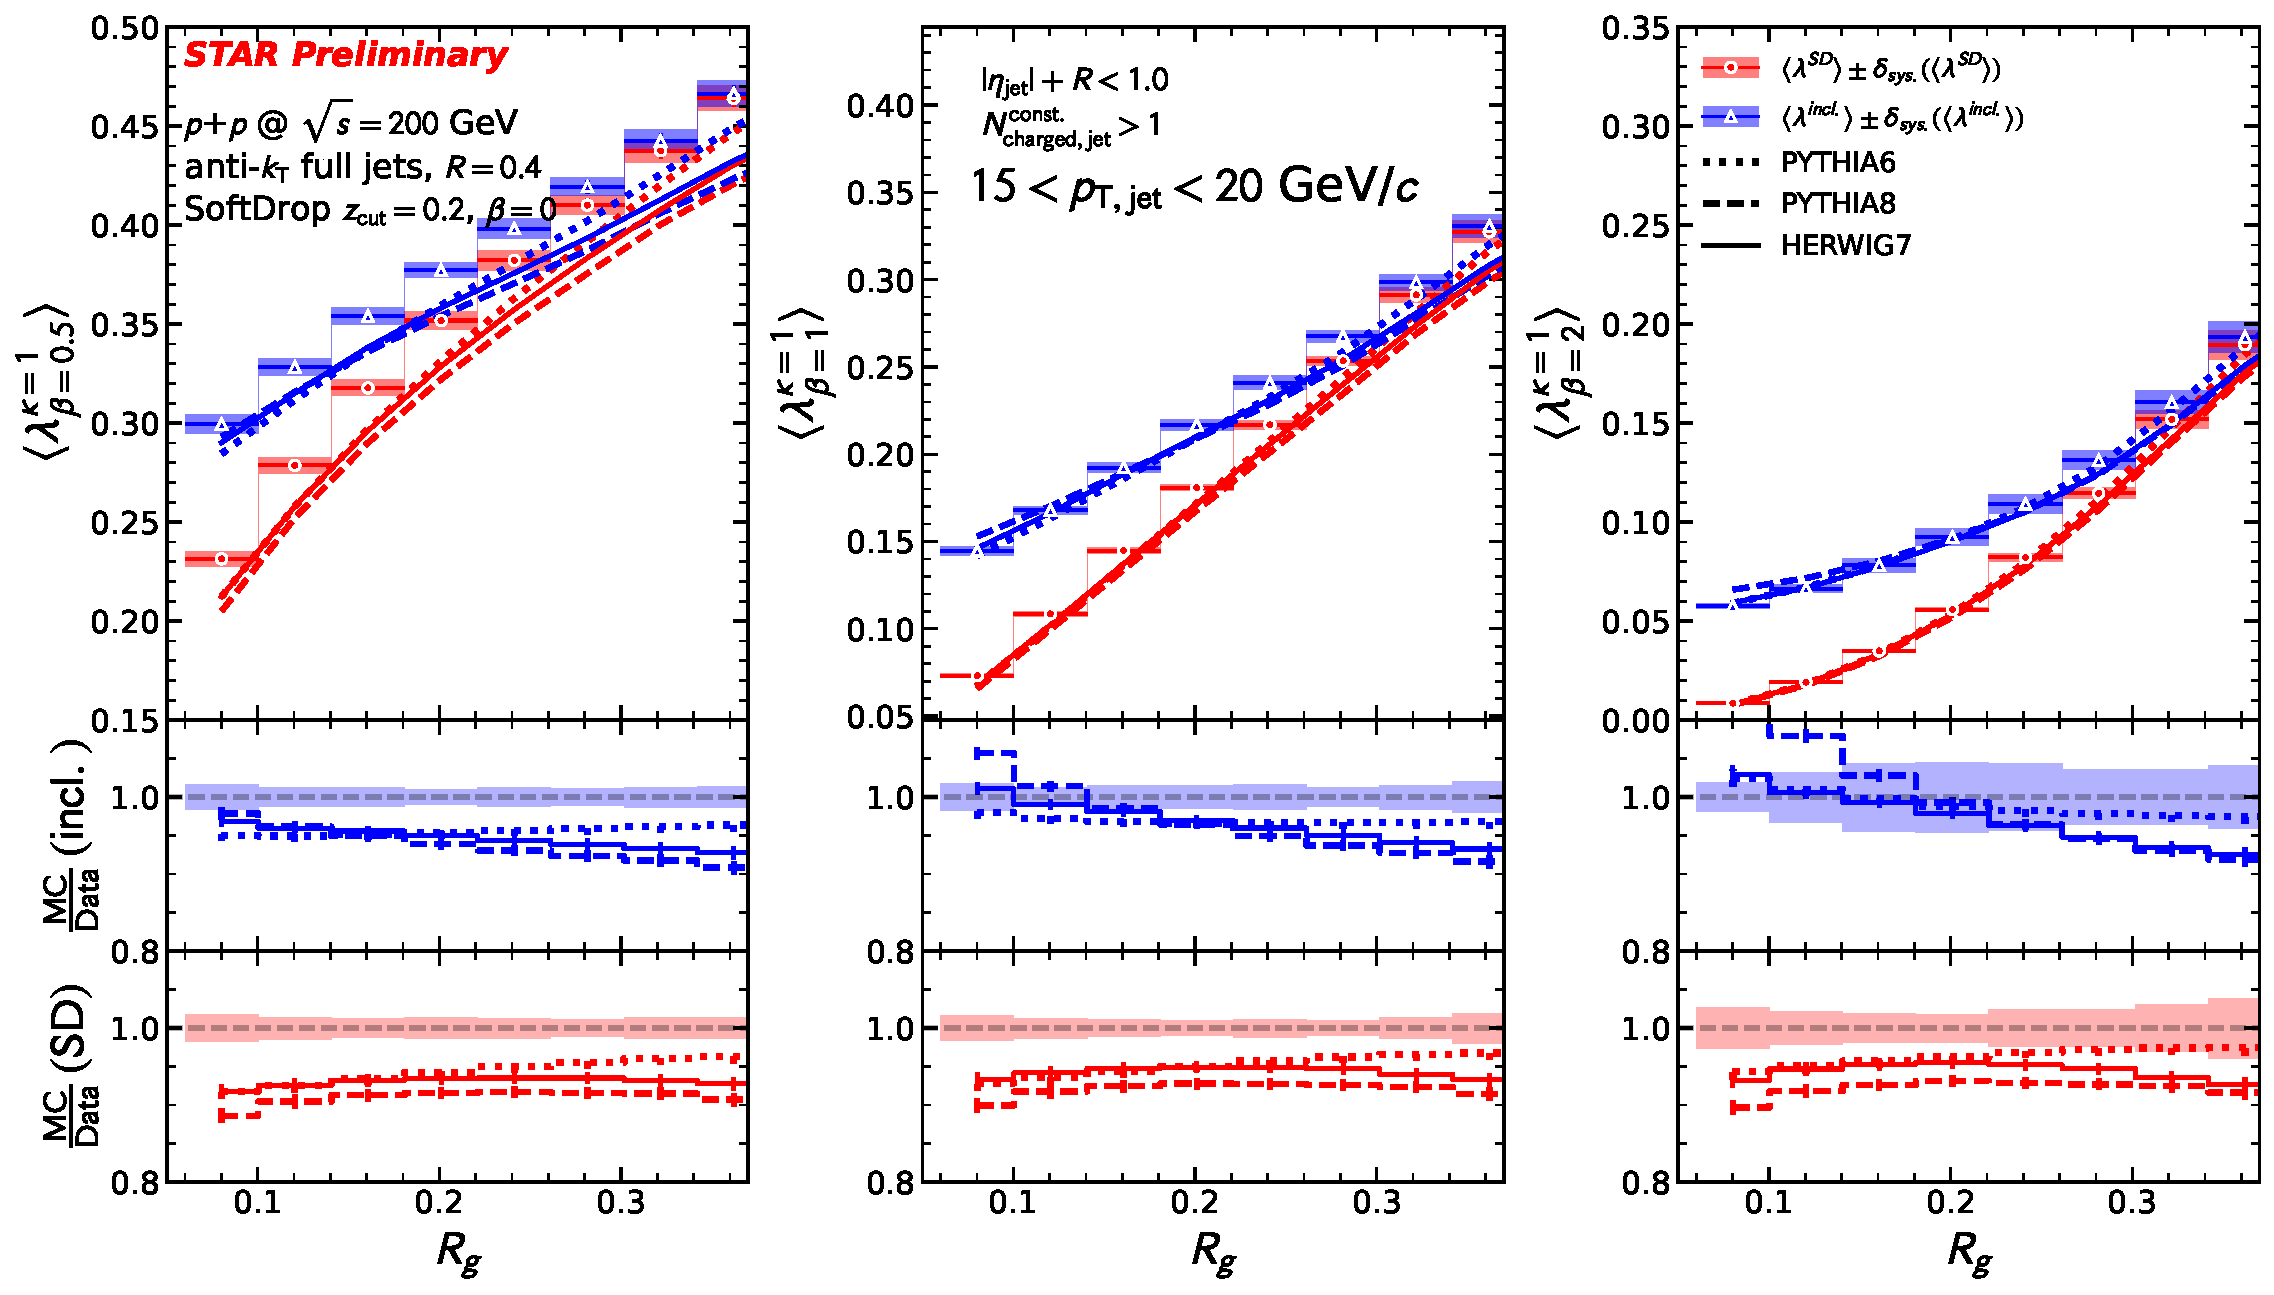
\includegraphics[width=\linewidth]{figures/fig_prof_grid_jpt1.pdf}
	\caption{Distributions of \(\lambda_\beta^1\) for \(\beta = 0\) (left), \(\beta = 1\) (middle) and \(\beta = 2\) (right) for jets with \ptRange{jet}{15}{20}. }
\end{figure}

\begin{figure}[h]
	\centering
	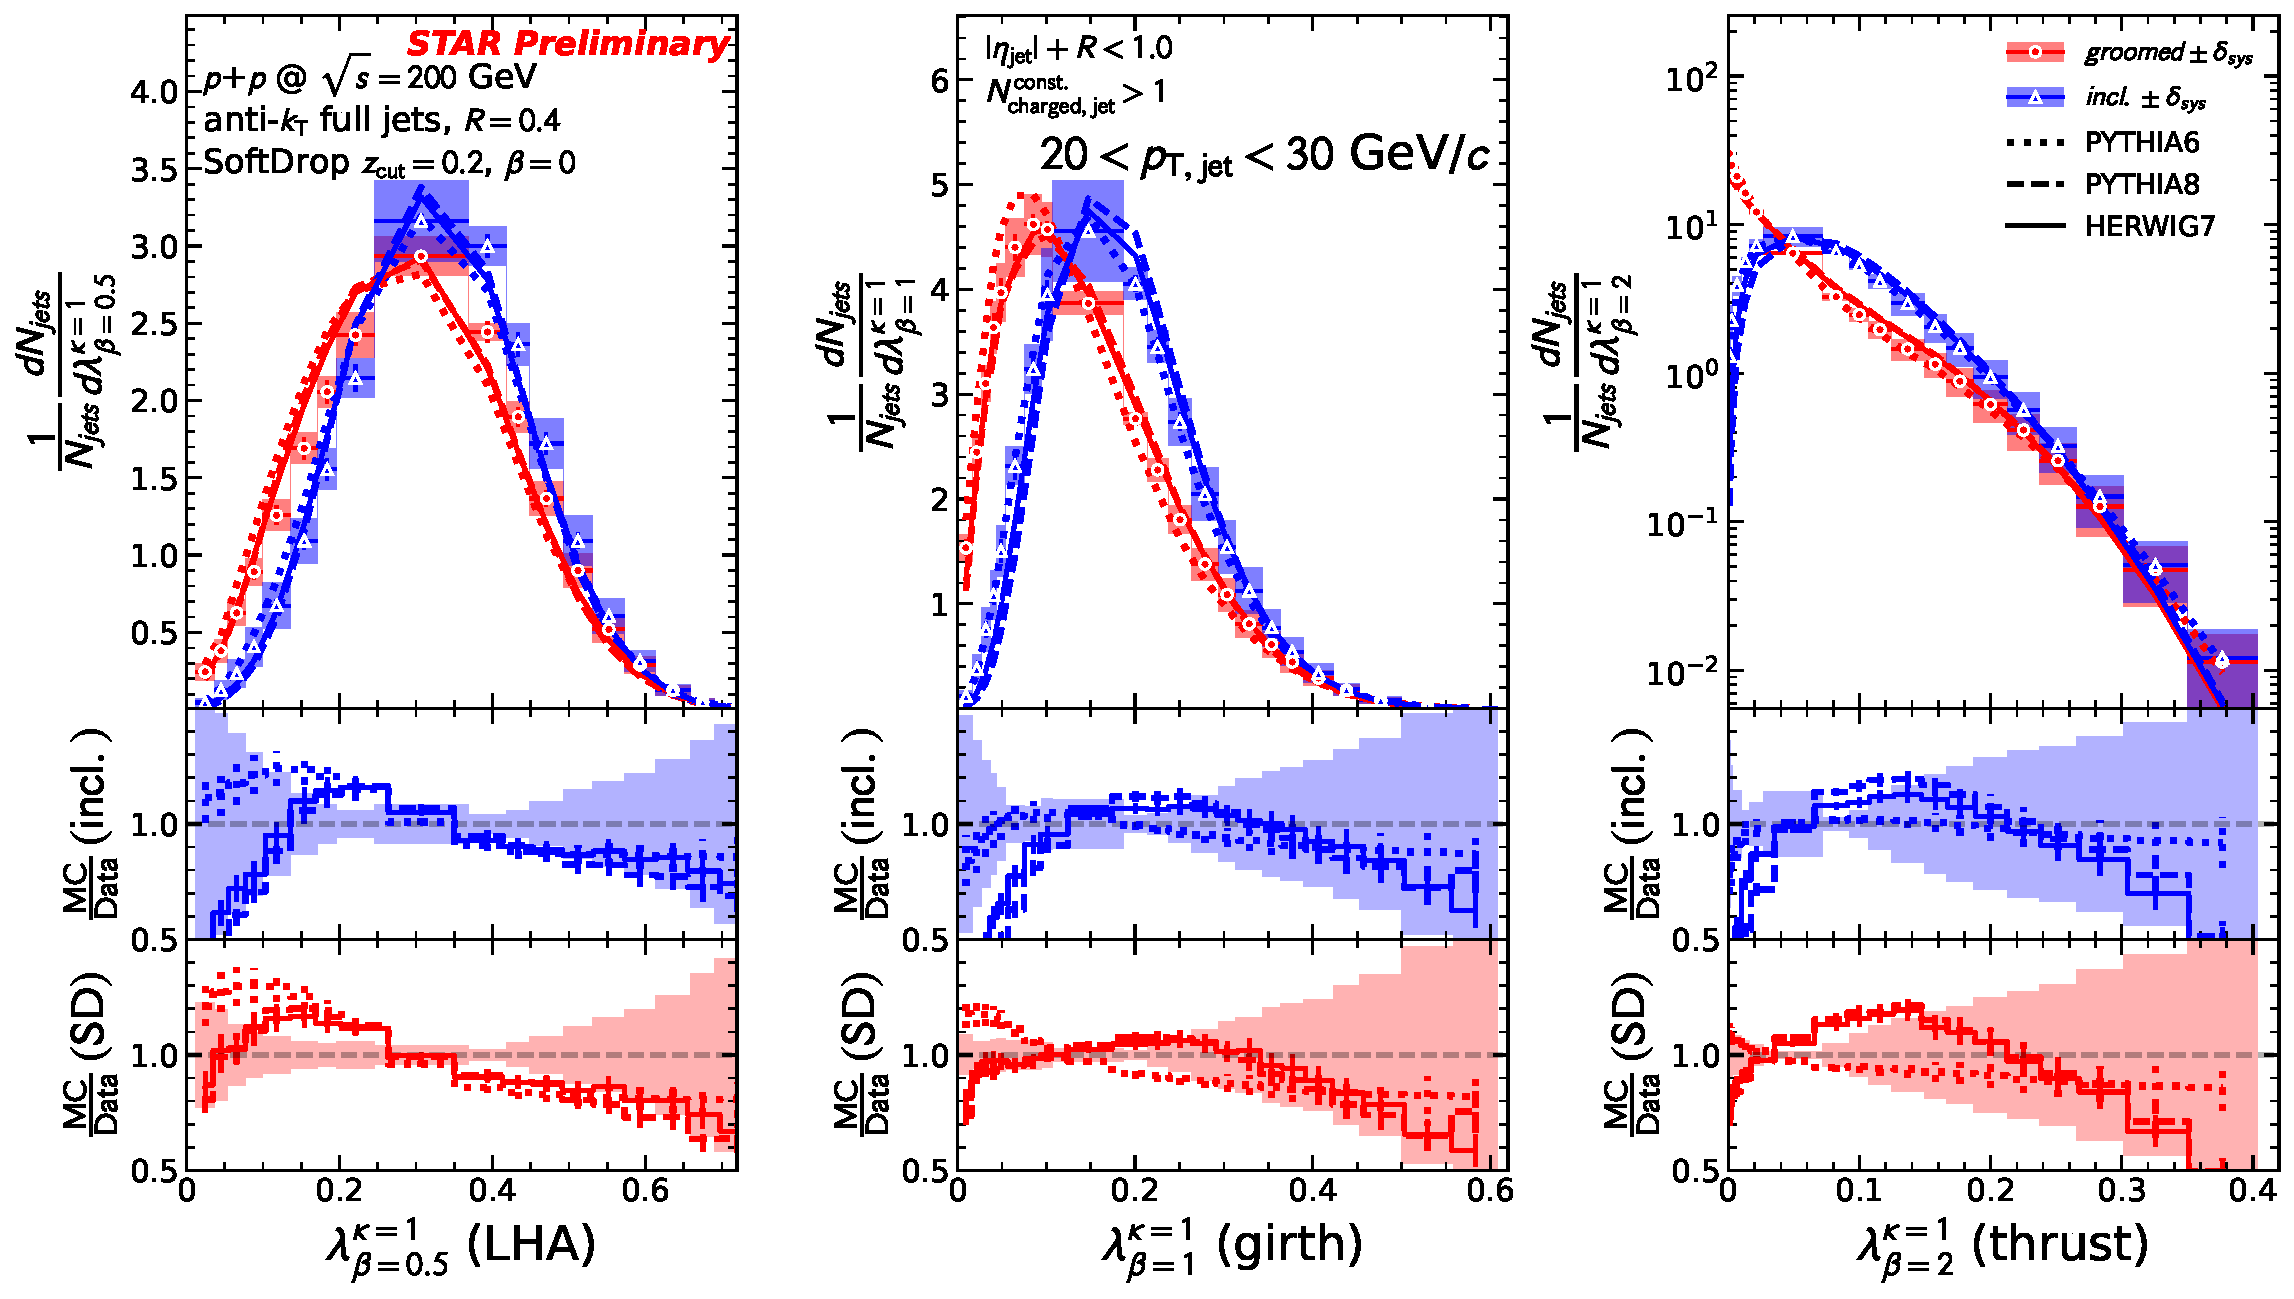
\includegraphics[width=\linewidth]{figures/fig_grid_jpt2.pdf}
			\caption{Distributions of \(\lambda_\beta^1\) for \(\beta = 0\) (left), \(\beta = 1\) (middle) and \(\beta = 2\) (right) for jets with \ptRange{jet}{20}{30}. }
\end{figure}
\begin{figure}[h]
	\centering
	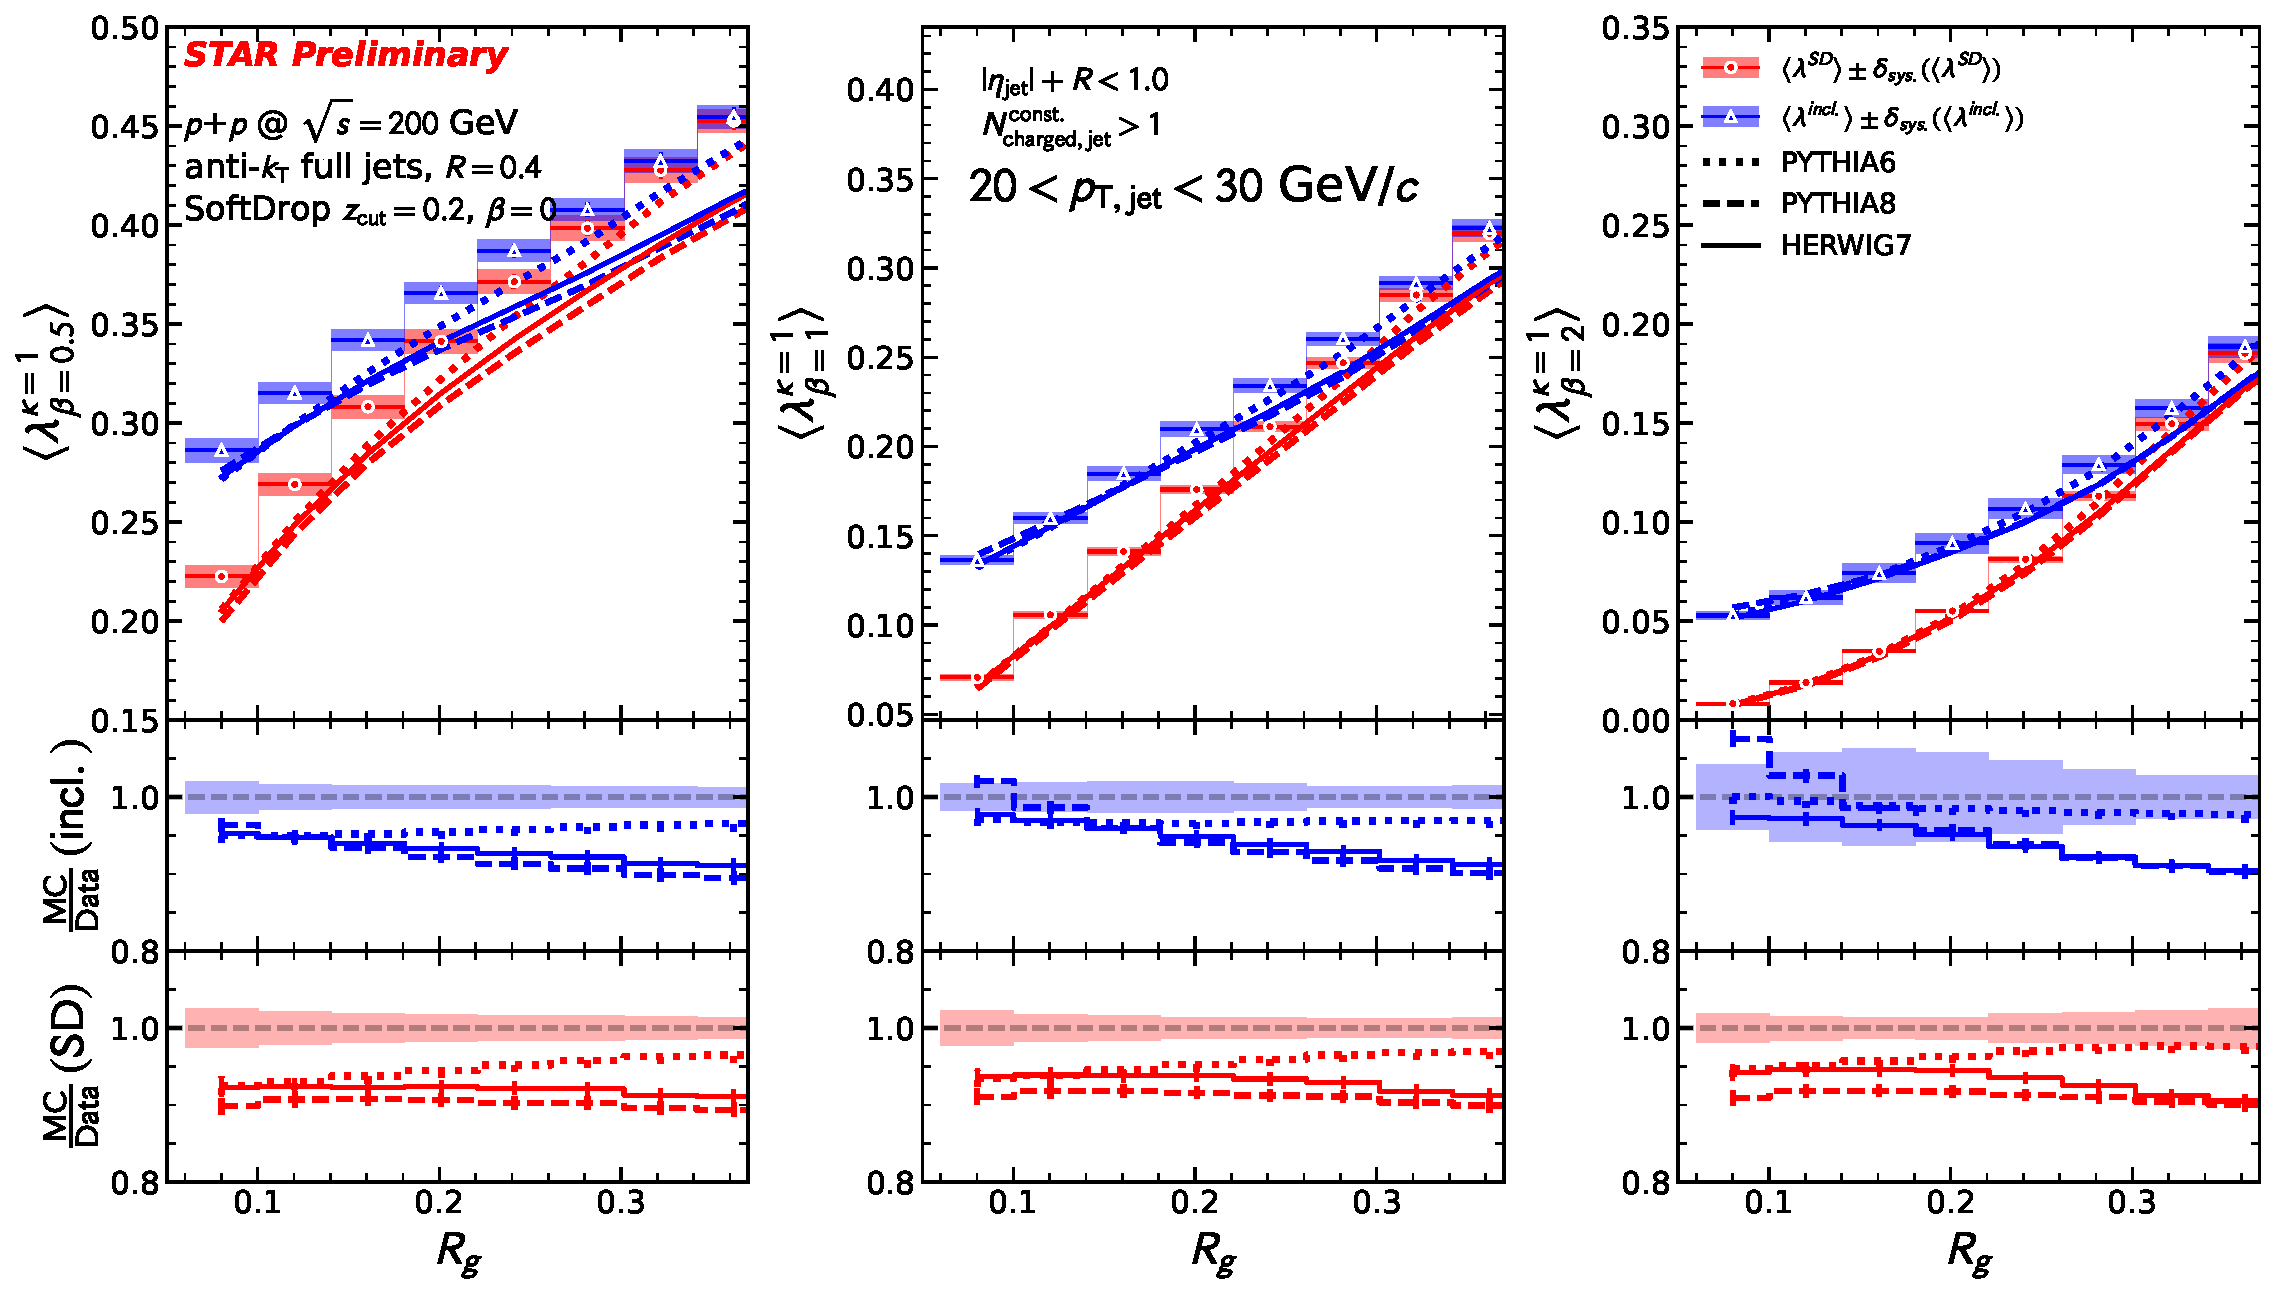
\includegraphics[width=\linewidth]{figures/fig_prof_grid_jpt2.pdf}
	\caption{Distributions of \(\lambda_\beta^1\) for \(\beta = 0\) (left), \(\beta = 1\) (middle) and \(\beta = 2\) (right) for jets with \ptRange{jet}{20}{30}. }
\end{figure}

\begin{figure}[h]
	\centering
	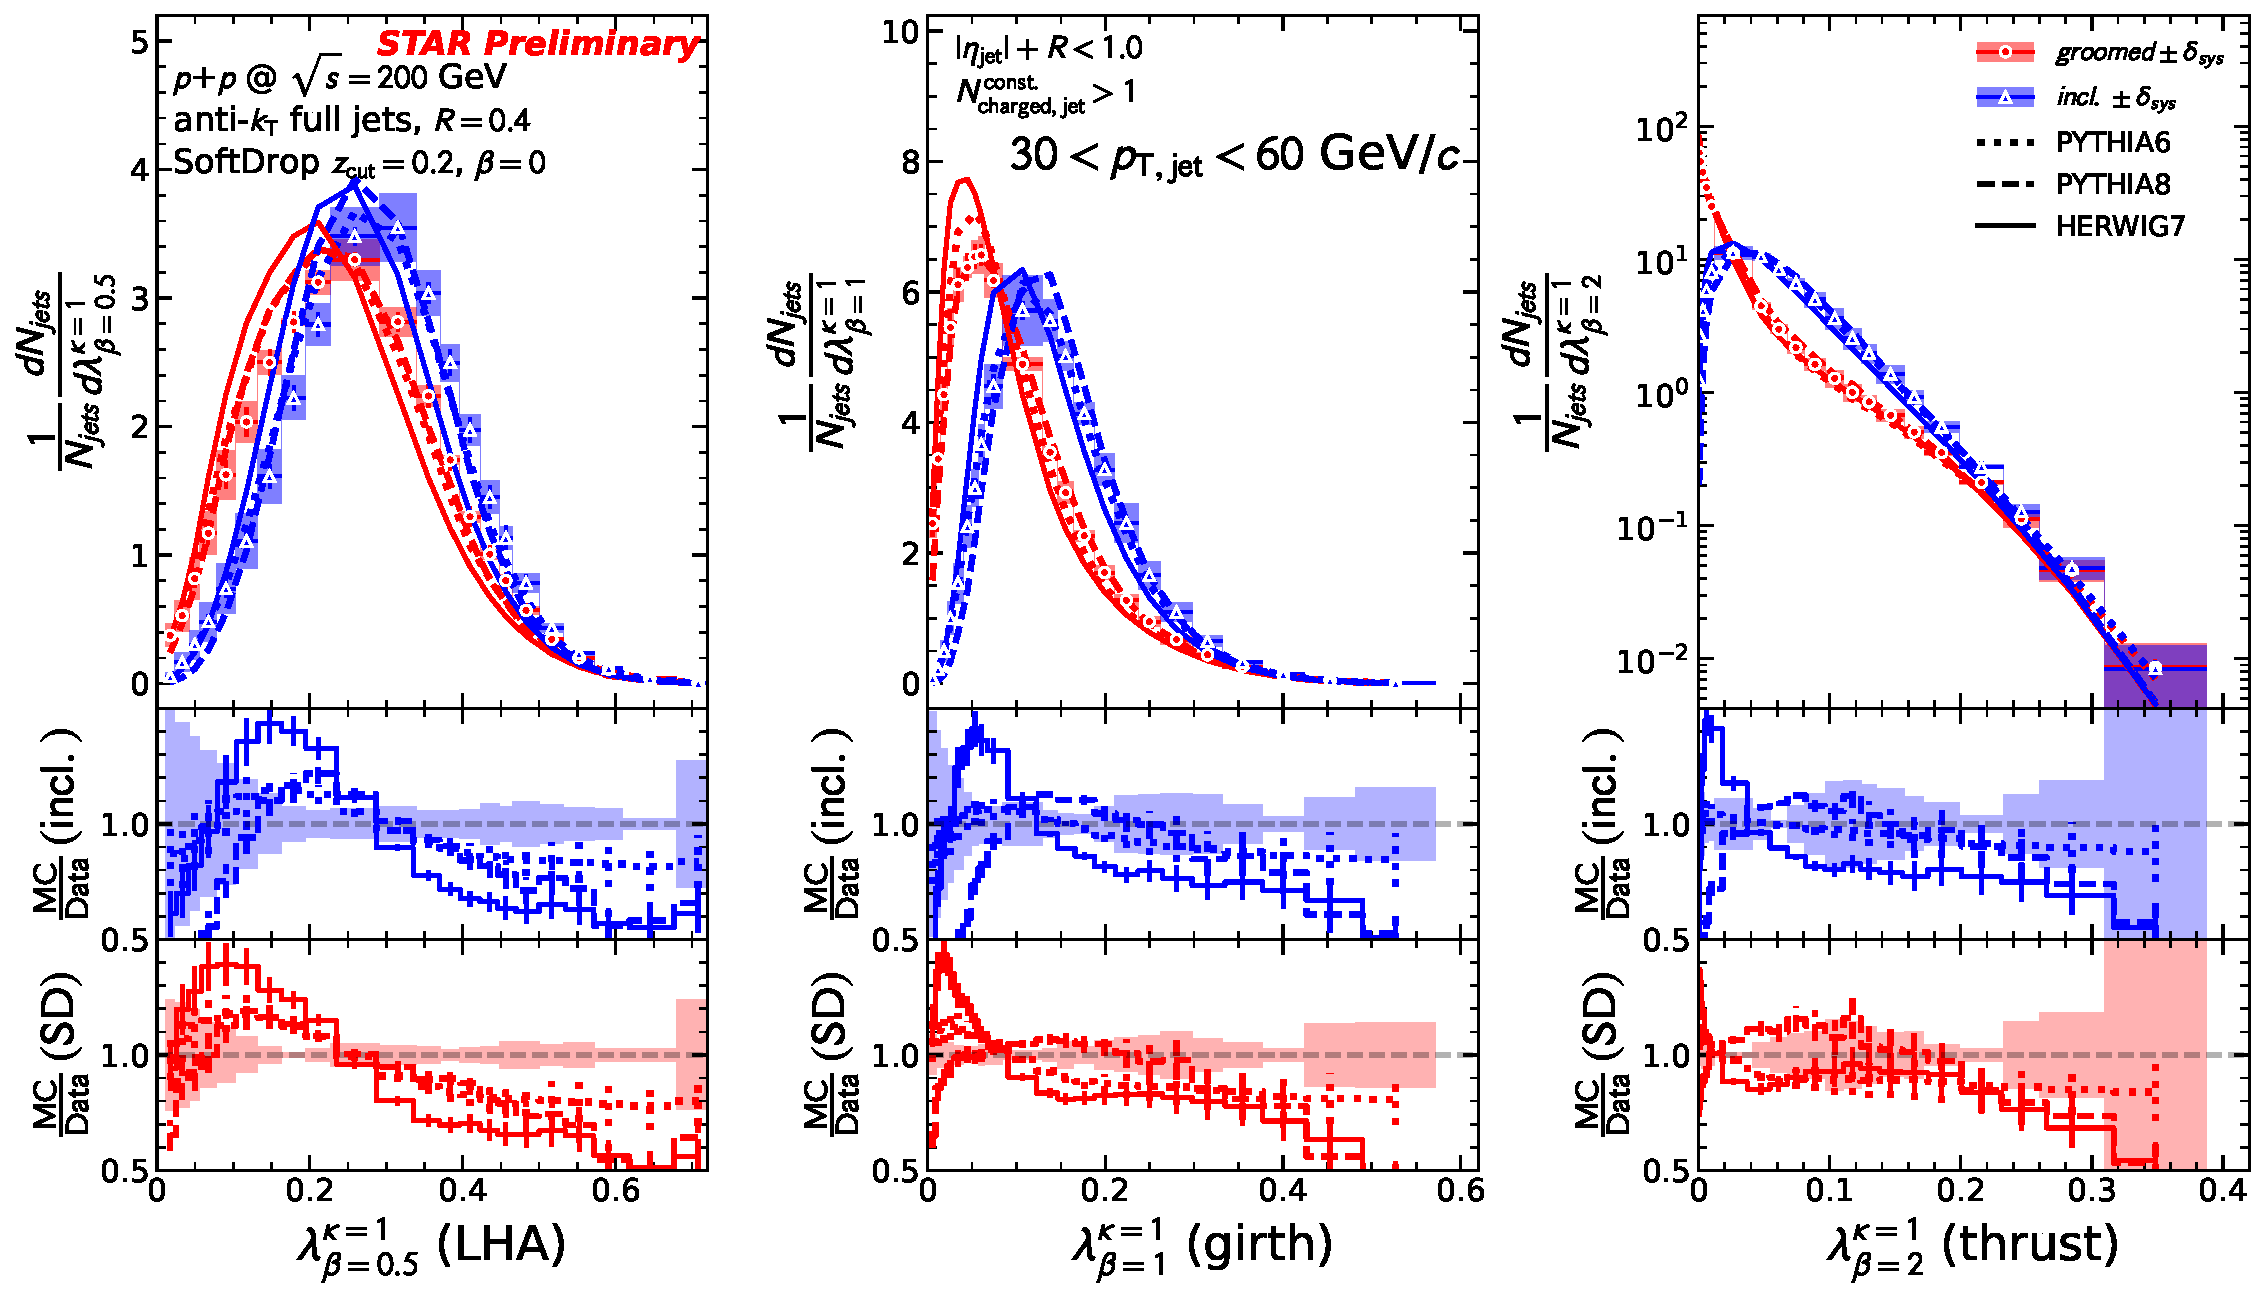
\includegraphics[width=\linewidth]{figures/fig_grid_jpt3.pdf}
			\caption{Distributions of \(\lambda_\beta^1\) for \(\beta = 0\) (left), \(\beta = 1\) (middle) and \(\beta = 2\) (right) for jets with \ptRange{jet}{30}{60}. }
\end{figure}
\begin{figure}[h]
	\centering
	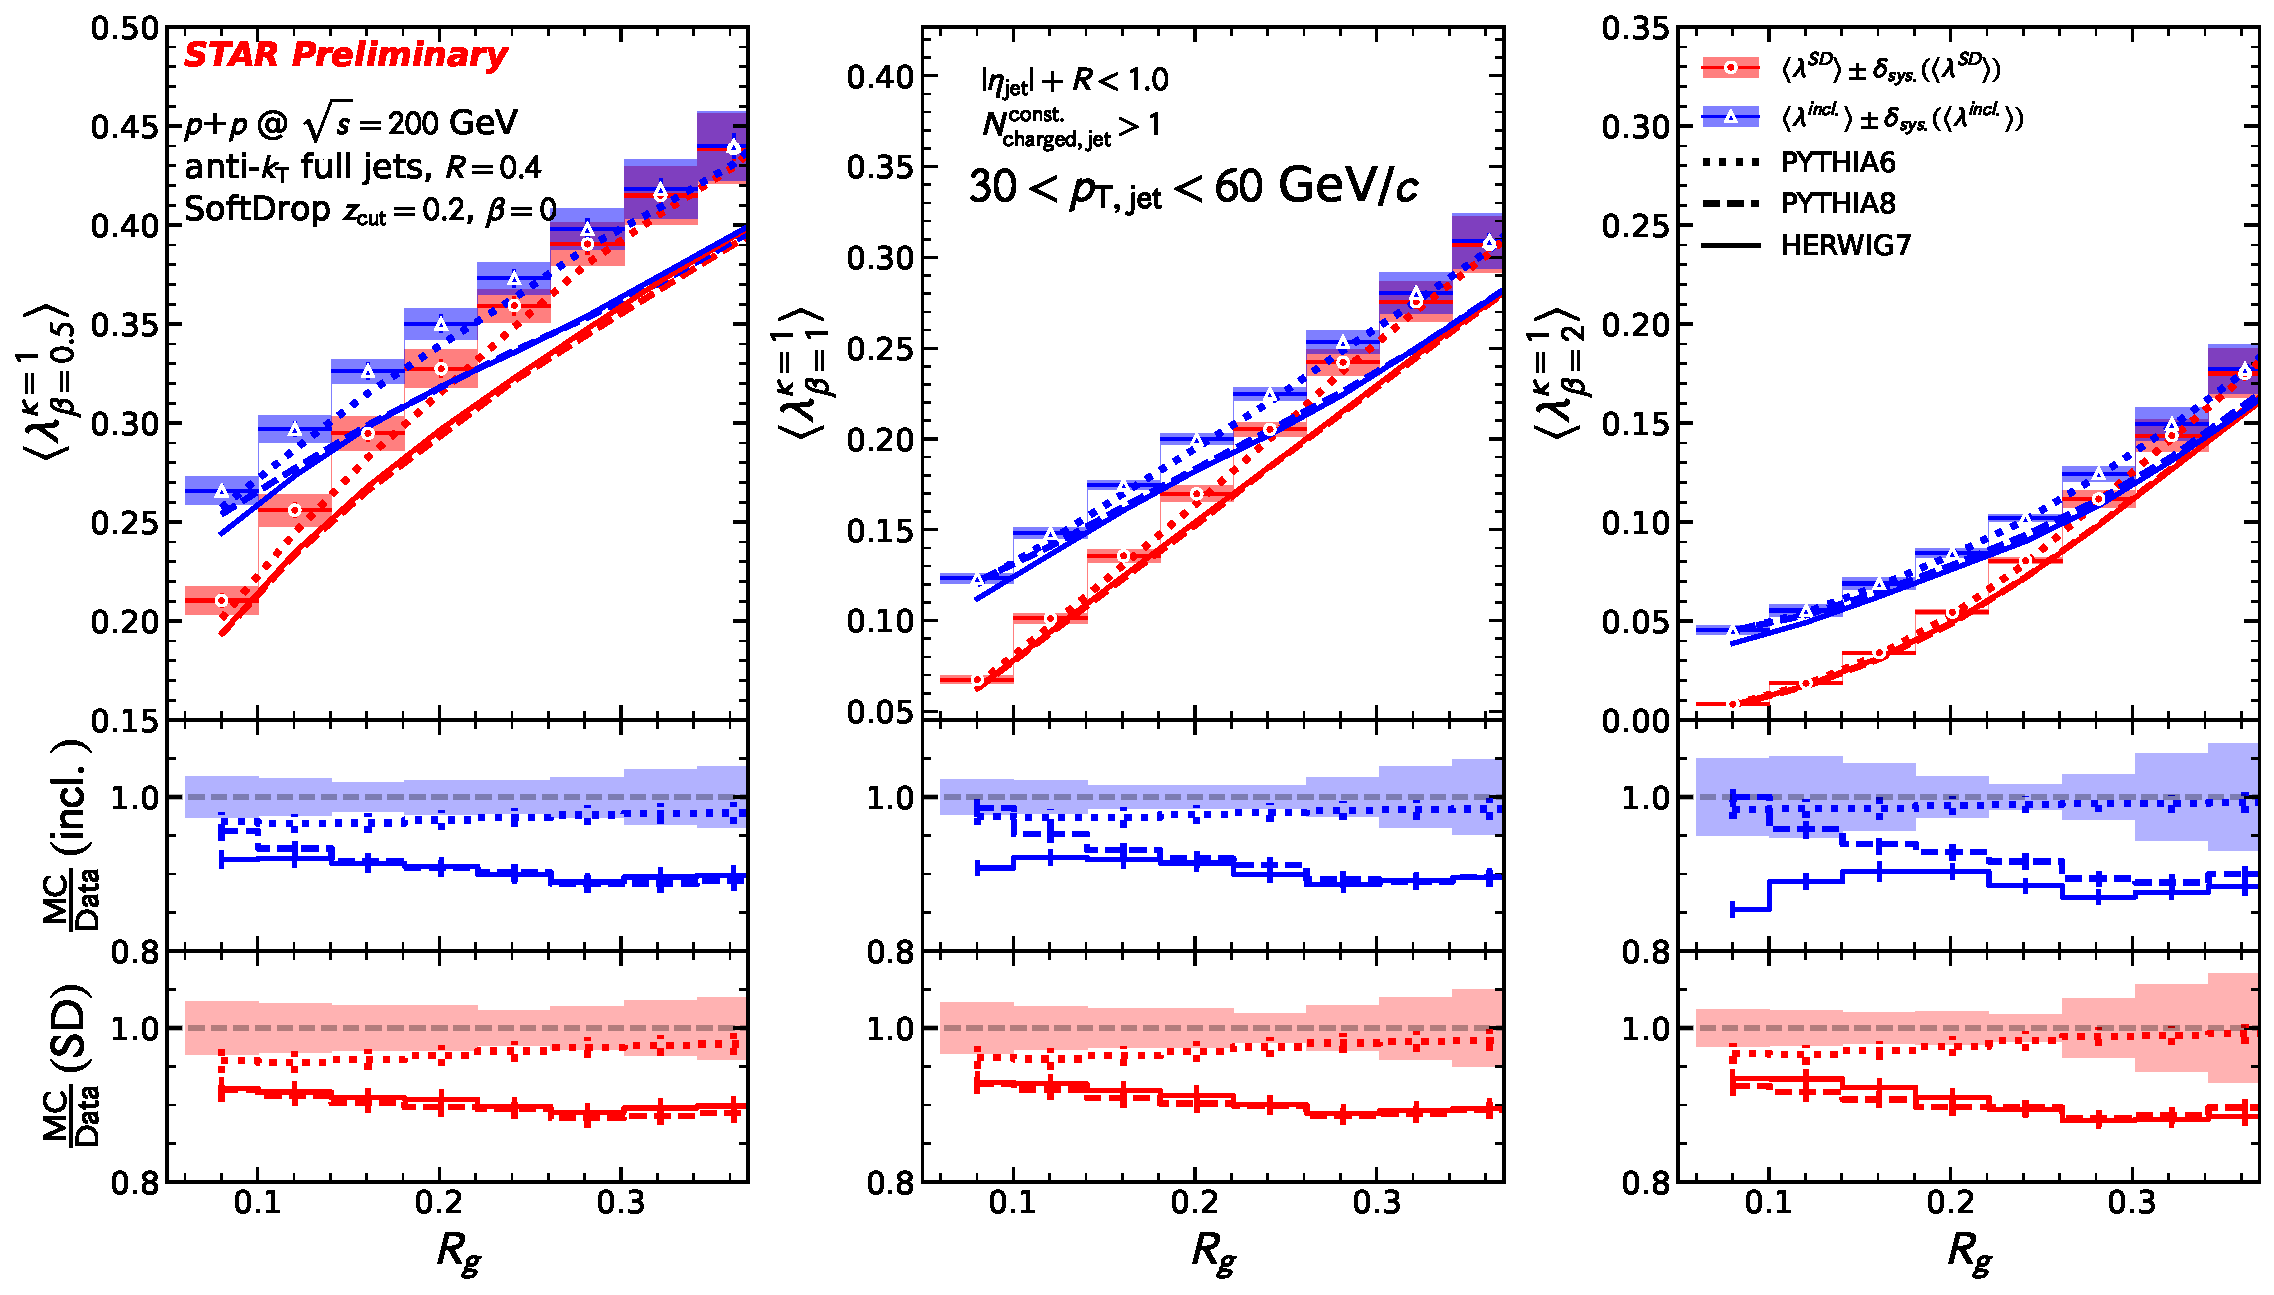
\includegraphics[width=\linewidth]{figures/fig_prof_grid_jpt3.pdf}
	\caption{Distributions of \(\lambda_\beta^1\) for \(\beta = 0\) (left), \(\beta = 1\) (middle) and \(\beta = 2\) (right) for jets with \ptRange{jet}{30}{60}. }
\end{figure}


\section{Angularities of Au+Au jets}
Charged-particle tracks and neutral energy depositions (towers) are measured using STAR's Time Projection Chamber (TPC) \cite{Anderson_2003} and Barrel Electromagnetic Calorimeter (BEMC) \cite{BEDDO2003725} detectors respectively. Together, they provide full azimuthal coverage with a pseudorapidity acceptance of $|\eta| \leq 1$.  The tracks and towers are clustered into jets using the anti-$k_{\rm T}$ algorithm with a jet resolution parameter $R = 0.4$, implemented using the FastJet library~\cite{Cacciari_2012}. To suppress contributions of fake tracks and combinatorial background (especially in the context of the larger  heavy-ion background), a ``hard-core'' constituent selection  is applied, as was done in previous STAR analyses \cite{PhysRevC.105.044906}, which only allows tracks (towers) with $cp_\mathrm{T, trk} (E_\mathrm{T, tow}) \geq 2~\mathrm{GeV}$ to be clustered into jets. To enhance jet signal, only High-Tower (HT) triggered events, with at least one tower with $\EtTower \geq 5.4$ GeV are considered. After clustering, only jets completely falling within acceptance ($|\eta_{\rm jet}| \leq 0.6$) are kept. Jets with area, $A_{\rm jet} < 0.4$ are rejected to further reduce the fake jet contribution.

%\begin{figure}[h]
%	\centering
%	\includegraphics[width=0.8\linewidth]{fig1_1}
%	\caption{Comparison between MultiFold and RooUnfold shown for jet mass (M) measurement from STAR p+p collisions at $\sqrt{s} = 200$ GeV, in \ptJet~ranges of \ptJetRange{20}{25} (left), \ptJetRange{25}{30} (middle), and \ptJetRange{30}{40} (right) \cite{song2023measurement}.}
%	\label{youqiFig}
%\end{figure}

Residual background and detector effects are removed by using a mapping between particle and detector level jets from an embedding simulation which involves PYTHIA-6 STAR tune \cite{adkins2019studying} events processed into detector hits using GEANT3 \cite{Brun:1987ma} and added to real minimum-bias events from Au+Au collision environment. MultiFold~\cite{PhysRevLett.124.182001} method was used to simultaneously unfold $p_{\rm T, jet}$, $\eta_{\rm jet}$, $\phi_{\rm jet}$, $N_{\rm cons, charged}$, \(g\), \(p_\mathrm{T}^\mathrm{D}\)~and LeSub. MultiFold uses Dense Neural Networks (DNNs) implemented using the EnergyFlow package~\cite{Komiske_2018},  which are trained on full embedding sample at the detector level and the generator level. Closure of the MultiFold is a measure of confidence in the algorithm determined by applying a pre-trained MultiFold on a detector level jet sample for which the particle level is known and comparing the two through ratios. Proper closure is demonstrated in Fig.\ref{fig:closure} for the obervables studied in these proceedings, with the ratios of distributions being consistent with unity within statistical errors.

\begin{figure}[h]
	\centering
	
\includegraphics[width=\linewidth]{closure_cent0to20_v3}
	\caption{Closure test for \(g\), \(p_\mathrm{T}^\mathrm{D}\)~and LeSub showing the ratio of distributions calculated using jets from unfolded 0-20\% centrality detector level and particle level events from Au+Au collisions at \sNN{200}{GeV}.}
	\label{fig:closure}
\end{figure}

%This study is the first instance of the MultiFold method being used to deconvolute detector effects from heavy-ion collision events.

\subsection{Result and Discussion}
Fully corrected measurements of \(g\), \(p_\mathrm{T}^\mathrm{D}\)~and LeSub distributions calculated from jets with $p_\mathrm{T, jet} > 20 \text{GeV}/c$ from events within centrality ranges of 0-20\% (central) and 40-80\% (peripheral), and ratio comparisons between distributions from  central and peripheral events are shown in Fig.~\ref{fig:JSO_Girth},~\ref{fig:JSO_PtD},~\ref{fig:JSO_LeSub} respectively. 
%
The \(p_\mathrm{T}^\mathrm{D}\)~distribution shows a discontinuity at 0.7 due to the strong dependence on number of constituents in jet. 
%
Systematic uncertainties were assumed to be uncorrelated, with uncertainties from various sources being added in quadrature.
%
Parameters varied for calculating the uncertainties in this study are the MultiFold regularization parameters of batch size and number of iterations. 
%
Any residual non-closure from MultiFold were also included in the calculation of systematic uncertainties. 
%
A prior variation uncertainty was added from previous calculations using STAR $\sqrt{s} = 200$ GeV p+p collision data. 

\begin{figure}[h]
	\centering
	\addOnePanelInFig{finalPlots_noPP_Girth_0_v3_warn.pdf}{0.495}
	\addOnePanelInFig{finalPlots_noPP_Girth_1_v3_warn.pdf}{0.495}
	\caption{Normalized \(g = \lambda_1^1\)  distributions for jets with \ptRange{jet}{15}{20} (left) and \ptGeq{jet}{20} (right) from central (0-20\%, red stars) and peripheral (40-80\%, blue stars) centrality ranges. Systematic uncertainties are shown as shaded boxes. Central over peripheral ratios (magenta stars) are in the lower panels with their systematic uncertainties represented as magenta boxes. Systematic uncertainties are assumed to be uncorrelated between the centrality ranges. }
	\label{fig:JSO_Girth}	
\end{figure}

\begin{figure}[h]
	\centering
	\addOnePanelInFig{finalPlots_noPP_PtD_0_v3_warn.pdf}{0.495}
		\addOnePanelInFig{finalPlots_noPP_PtD_1_v3_warn.pdf}{0.495}
	\caption{Normalized \(p_\mathrm{T}^\mathrm{D} = \sqrt{\lambda^2_0}\) distributions for jets with \ptRange{jet}{15}{20} (left) and \ptGeq{jet}{20} (right) from central (0-20\%, red stars) and peripheral (40-80\%, blue stars) centrality ranges. Systematic uncertainties are shown as shaded boxes. Central over peripheral ratios (magenta stars) are in the lower panels with their systematic uncertainties represented as magenta boxes. Systematic uncertainties are assumed to be uncorrelated between the centrality ranges. }
	\label{fig:JSO_PtD}	
\end{figure}

\begin{figure}[h]
	\centering
	\addOnePanelInFig{finalPlots_noPP_LeSub_0_v3_warn.pdf}{0.495}
	\addOnePanelInFig{finalPlots_noPP_LeSub_1_v3_warn.pdf}{0.495}
	\caption{Normalized LeSub distributions for jets with \ptRange{jet}{15}{20} (left) and \ptGeq{jet}{20} (right) from central (0-20\%, red stars) and peripheral (40-80\%, blue stars) centrality ranges. Systematic uncertainties are shown as shaded boxes. Central over peripheral ratios (magenta stars) are in the lower panels with their systematic uncertainties represented as magenta boxes. Systematic uncertainties are assumed to be uncorrelated between the centrality ranges. }
	\label{fig:JSO_LeSub}	
\end{figure}
Results are consistent between central and peripheral collisions within conservative systematic uncertainties. This can be attributed to the assumption of uncorrelated systematic uncertainties, and a bias in the analysis towards hard-fragmented jets due to the selection of events and constituents for jet clustering. Harder-fragmented jets, on average are narrower and have lower interaction time with QGP, which could make any relative modification in central events compared to the peripheral ones lower than what would be potentially observed in an inclusive jet analysis. 

\section{Conclusion and Outlook}
Inclusive and groomed angularities have been measured for \(p+p\)  collisions at \sPP{200}{GeV}. 
%
The distributions, presented in different \(p_\mathrm{T, jet}\) ranges show generally show good agreement with  PYTHIA-6, PYTHIA-8 and HERWIG-7 tuned to the RHIC energies.  
%
The \(R_\mathrm{g}\) profiles conform with expectations from QCD. This measurement will be used as baselines for the ongoing heavy-ion measurements. 
%

Measurements for \(g=\lambda_1^1\), \(p_T^D = \sqrt{\lambda_0^2}\) and LeSub done with hard-core jets from Au+Au collisions at \sNN{200}{GeV} show almost no quenching from \(R_\mathrm{CP}\) calculations discussed. 
%
However, that could have been due to the crude hard-core selections, introducing a survivor bias, and utilizing grooming going forward might be useful. 




